%24/02 - Aythami Morales 
\chapter{Aprendizaje supervisado}
\section{Introducción}
El aprendizaje automático se divide en dos grandes categorías: aprendizaje supervisado y aprendizaje no supervisado. En el aprendizaje supervisado, el objetivo es aprender una \textbf{función de hipótesis} desconocida que permita predecir una salida $y$ a partir de una entrada $x$. Este enfoque se conoce como sistema \textbf{data-driven}, ya que el modelo aprende patrones a partir de datos etiquetados.

\subsection{Datos etiquetados}
En el aprendizaje supervisado, cada dato tiene una etiqueta asociada, lo que se representa como pares $(x^{(i)}, y^{(i)})$. Partimos de un \textbf{conjunto de datos de entrenamiento}:
$$D_{train} = \{ (\vec{x}_n, y_n)\}^{N_{train}}_{n=1}$$
siendo:
\begin{itemize}
\item $N_{train}$: número de muestras de entrenamiento.
\item $\vec{x}_n$: vector de atributos (inputs, características, variables independientes).
\item $y_n$: etiqueta o valor objetivo.
\end{itemize}

El objetivo es \textbf{inducir o aprender} a partir de los datos de entrenamiento un \textbf{predictor} $h$ que permita predecir $y$ para nuevos datos. La clave no es memorizar los datos de entrenamiento, sino \textbf{generalizar} para hacer predicciones precisas en situaciones similares pero no idénticas (capacidad de generalización).

\subsection{Función de hipótesis y predictor}
El algoritmo de aprendizaje $L$ toma los datos de entrenamiento y busca una función $h$ que sirva como predictor:
$$L:D_{train} \rightarrow h$$
\begin{itemize}
\item $h$: función de hipótesis que mapea entradas $x$ a salidas $y$.
\item El predictor debe ser capaz de generalizar, es decir, funcionar bien con datos no vistos durante el entrenamiento.
\end{itemize}

\subsection{Tipos de problemas en aprendizaje supervisado}
\paragraph{Clasificación}
En un problema de clasificación, hay un espacio que se divide en las distintas etiquetas que adquieren los datos. No se trata de buscar la línea divisoria entre los distintos elementos, si no la caracterización de los espacios en los que se encuentran. Esa línea divisoria, o frontera de decisión, es importante para dicha caracterización. La salida es discreta, ya que se trata de etiquetas categóricas. Puede ser binaria (dos clases) o multiclase, pero nunca un dato podrá estar entre dos etiquetas. Además, las etiquetas pueden seguir un orden (etiqueta 1 < etiqueta 2 < etiqueta 3) o no.

\paragraph{Regresión}
Un ejemplo es la predicción del tamaño de un tumor en función del tiempo que lleva desarrollándose mediante la descripción de la tasa de crecimiento. En este caso, los datos son el tiempo (distinto número de semanas) y las etiquetas el tamaño del tumor, y se busca describir el tamaño para datos nuevos, como pueden ser semanas no descritas. Aun así, para una misma semana, puede haber distintas tasas de crecimiento dependiendo de la persona. En este caso sí se busca encontrar la recta. Puede haber varias soluciones independientes, y en este caso la salida es continua (un valor numérico).

El número máximo de clases a partir de que un problema pasa de clasificación a regresión depende de la naturaleza del problema. Si el problema es de naturaleza continua, entonces la aproximación será mediante regresión, mientras que si el problema es discreto, entonces utilizaremos la clasificación. Si existe una relación entre muestras consecutivas, se espera que una distancia entre muestras esté correlacionada o haya consecuencialidad. 

En resumen, en problemas de clasificación, el espacio de características se divide en regiones según las etiquetas. Por ejemplo, en un problema binario, se busca una frontera de decisión que separe las dos clases. En regresión, se busca una función (como una recta) que ajuste los datos.

\subsection{Función de pérdida}
Hasta ahora, seguíamos la siguiente notación:
\begin{itemize}
\item $x$, $y$: son variables aleatorias con una distribución conjunta, es decir, hay un patrón que permite predecir una variable en función de la otra.
\item Predictor $h$: permite obtener $y$ a partir de $x$.
\end{itemize}

La \textbf{función de pérdida} $L$ mide la discrepancia entre la predicción $h(x)$ y la etiqueta real $y$. El objetivo es minimizar esta pérdida. Existen dos tipos comunes de funciones de pérdida:
\begin{enumerate}
\item Clasificación
\begin{itemize}
\item Pérdida 0-1: 
$$L(h(x),y) = \mathbb{I}(h(x) \neq y)$$

donde $\mathbb{I}$ es una función indicadora que vale 1 si la predicción es incorrecta y 0 si es correcta. Así, el error se calcula como la suma de las predicciones incorrectas. Un sistema que acierte mucho tendrá un indicador $\mathbb{I}$ cercano a 0, mientras que un sistema que falle mucho tendrá un $\mathbb{I}$ alto que habrá que normalizar por los intentos realizados.
\end{itemize}

\item Regresión
\begin{itemize}
\item Error cuadrático medio (MSE):
$$MSE = \mathbb{E}[|h(\vec{X}) - Y|^2]$$

\item Error absoluto medio (MAE):
$$MAE = \mathbb{E}[|h(\vec{X}) - Y|]$$

\item El MSE magnifica los errores grandes debido al cuadrado, mientras que el MAE es más robusto y mantiene el sentido físico-biológico de la variable.
\end{itemize}
\end{enumerate}

\subsection{Pérdida esperada y generalización}
La pérdida esperada es un estimador que mide el rendimiento del modelo en toda la población, no solo en los datos de entrenamiento. Esto se debe a que los datos de entrenamiento se definen en una subregión o espacio finito de la región de todos los posibles valores. Se busca que el entrenamiento tenga un rendimiento bueno con datos conocidos y desconocidos. Se define como:
$$Error = \mathbb{E}[\mathbb{I}(h(\vec{X}) \neq Y)]$$

El objetivo es minimizar la pérdida esperada, lo que implica que el modelo generalice bien a datos nuevos.

\subsection{Entrenamiento y optimización}
El entrenamiento consiste en ajustar los \textbf{parámetros} $\Theta$ del modelo para minimizar la pérdida en los datos de entrenamiento. La pérdida promedio en el conjunto de entrenamiento se define como:
$$L_{train}(\Theta) = \frac{1}{N_{train}} \sum^{N_{train}}_{n=1} L(h(\vec{x}^{train}_n; \Theta), y^{train}_n)$$
\begin{itemize}
\item $\Theta$: parámetros del modelo (por ejemplo, coeficientes en regresión lineal).
\item $L_{train}$: pérdida promedio en el conjunto de entrenamiento.
\end{itemize}

Sin embargo, minimizar $L_{train}$ no garantiza un buen rendimiento en datos nuevos. Esto se debe al \textbf{sobreajuste} (overfitting), donde el modelo memoriza los datos de entrenamiento pero no generaliza bien a datos no vistos.

Para evitar el sobreajuste, se introduce una \textbf{penalización de complejidad} en la función de pérdida. Esto limita el número de parámetros o la magnitud de los mismos, favoreciendo modelos más simples y generalizables. Ejemplos comunes incluyen la regularización L1 (Lasso) y L2 (Ridge) que penalizan la suma absoluta o cuadrática de los parámetros respectivamente.

\subsubsection{Sesgos en el entrenamiento}
La pérdida de entrenamiento suele ser menor que la pérdida en datos nuevos, ya que el modelo se optimiza específicamente para los datos de entrenamiento. Esto introduce un \textbf{sesgo} en el proceso de entrenamiento. Para evaluar el rendimiento del modelo en datos no vistos, se utiliza un \textbf{conjunto de test}:

Los datos de test no se usan para ajustar $\Theta$, solo para evaluar el rendimiento. La pérdida en el conjunto de test se calcula de manera similar a $L_{train}$, pero sin modificar $\Theta$.

%25/02 - Aythami
\paragraph{Underfitting}
El tipo de predictor considerado tiene \textbf{poca capacidad expresiva} o pocos grados de libertad. En consecuencia, no es capaz de capturar las dependencias entre los atributos y la variable a predecir. La pérdida esperada del predictor es demasiado elevada. Esto suele ocurrir en modelos rígidos, como pueden ser los modelos lineales.

\paragraph{Overfitting}
El tipo de predictor considerado es \textbf{demasiado flexible} (demasiados grados de libertad) y aprende patrones espurios que no son relevantes para la predicción (por ejemplo, fluctuaciones de muestreo, ruido, valores atípicos, etc.). La estimación de entrenamiento de la pérdida esperada es demasiado optimista y subestima la pérdida esperada real. Esto puede ocurrir en modelos flexibles, como pueden ser las redes neuronales.

\begin{figure}[h]
\centering
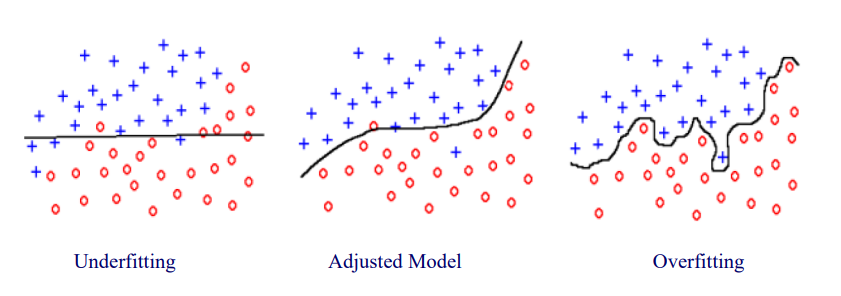
\includegraphics[width = 0.8\textwidth]{figs/under-overfitting.png}
\end{figure}

\subsection{Compensación entre sesgo y varianza}
Se tiene un sesgo bajo en modelos flexibles que se ajustan bien a los datos de entrenamiento, pero pueden tener alta varianza (sobreajuste). El sesgo alto se suele dar en modelos rígidos que no se ajustan bien a los datos, pero tienen baja varianza (underfitting). Por ello, se describe la compensación. A medida que aumenta la complejidad del modelo, el error de entrenamiento disminuye, pero el error de test puede aumentar después de un punto óptimo debido al sobreajuste.

\begin{figure}[h]
\centering
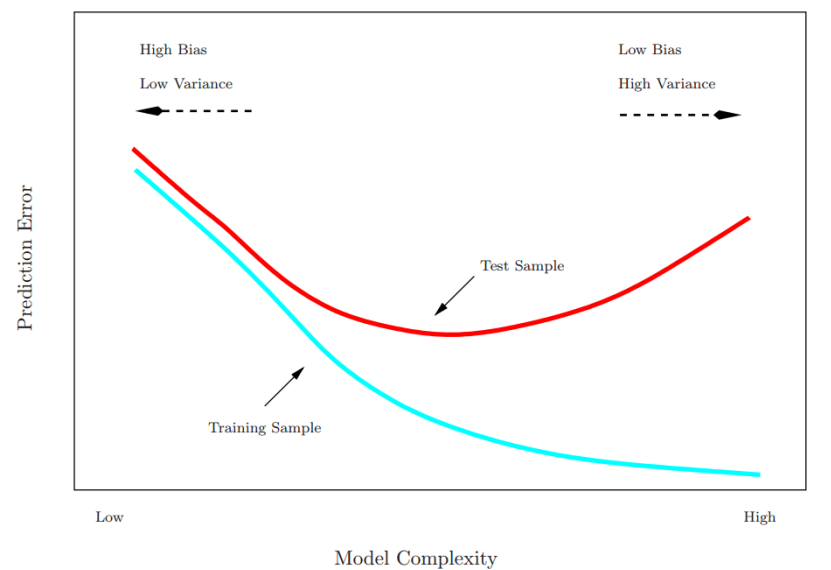
\includegraphics[width = 0.8\textwidth]{figs/tradeoff.png}
\caption{En el eje x está la complejidad del modelo, o el orden del polinomio. En el eje y está la predicción del error. Se empieza con un error alto, y se va adaptando, mediante modelos más complejos, para disminuir el error. No obstante, llega un momento en el que, aunque el error de entrenamiento siga bajando con modelos cada vez más complejos, el error de test vuelve a aumentar, indicando un modelo sobreajustado.}
\end{figure}

\subsection{Arquitectura, parámetros}
\begin{itemize}
\item \textbf{Arquitectura, configuración}: Especificación de la forma funcional del predictor (por ejemplo, número y tipo de capas ocultas y neuronas en una red neuronal, elección del núcleo en una SVM, etc.). En el caso de la regresión polinomial, es el polinomio.
\item \textbf{Parámetros del modelo} $\Theta$: Valores necesarios para especificar el sistema de predicción (por ejemplo, pesos sinápticos en una red neuronal, vectores de soporte en una SVM, etc.). Se determinan entrenando el modelo con datos etiquetados.
\item \textbf{Configuración del algoritmo de aprendizaje}: Función a optimizar (por ejemplo, verosimilitud, probabilidad posterior, error cuadrático medio, etc.). Términos de regularización
\end{itemize}

Hay distintos tipos de modelos predictivos: vecinos cercanos, árboles de decisión, redes neuronales, Support Vector Machine.

\subsection{Preprocesado de datos}
El preprocesado es crucial para preparar los datos antes de entrenar un modelo. Incluye:
\begin{enumerate}
\item \textbf{Selección de características}: identificar las características más relevantes
\item \textbf{Manejo de valores atípicos (outliers)}: detectar y tratar datos anómalos
\item \textbf{Manejo de datos faltantes}: imputar o eliminar valores faltantes
\item \textbf{Normalización}: centrar y escalar los datos para que tengan media 0 y desviación estándar 1. La normalización basada en la media y desviación estándar es más robusta que usar valores mínimos y máximos.
\end{enumerate}

El preprocesado se puede realizar programáticamente con el módulo de scikit-learn.

\subsection{Medición del rendimiento}
\subsubsection{Error de clasificación}
El error de clasificación se estima como la proporción de veces que el modelo predice incorrectamente las etiquetas. Es una métrica básica para evaluar la efectividad del modelo.

\subsubsection{Matriz de confusión}
La matriz de confusión es una herramienta fundamental para evaluar el rendimiento en problemas de clasificación. Muestra las combinaciones entre las etiquetas reales y las predichas. En clasificación binaria, se divide en:
\begin{itemize}
\item \textbf{True Positive (TP)}: correctamente clasificados como positivos.
\item \textbf{True Negative (TN)}: correctamente clasificados como negativos.
\item \textbf{False Positive (FP)}: incorrectamente clasificados como positivos.
\item \textbf{False Negative (FN)}: incorrectamente clasificados como negativos.
\end{itemize}

En problemas con más de dos clases, la matriz de confusión se extiende, y la diagonal principal indica las predicciones correctas, mientras que las demás celdas muestran los errores. Esto es útil para identificar qué clases se confunden con mayor frecuencia.

\subsubsection{Métricas de rendimiento}
A partir de la matriz de confusión, se derivan varias métricas para evaluar el rendimiento del modelo:
\begin{itemize}
\item \textbf{Accuracy (exactitud)}: mide la efectividad general del modelo.
$$Accuracy = \frac{TP + TN}{TP + TN + FP + FN}$$

\item \textbf{Error}: estimación de la proporción de clasificación incorrectas.
$$Error = 1 - Accuracy = \frac{FP + FN}{TP + TN + FP + FN}$$

\item \textbf{Sensitividad (Recall)}: ratio de positivos correctamente identificados.
$$Sensitividad = \frac{TP}{TP + FN}$$

\item \textbf{Especifidad}: ratio de negativos correctamente identificados.
$$Especificidad = \frac{TN}{TN + FP}$$

\item \textbf{Precisión}: ratio de predicciones positivas que son correctas.
$$Precision = \frac{TP}{TP + FP}$$
\end{itemize}

\begin{figure}[h]
\centering
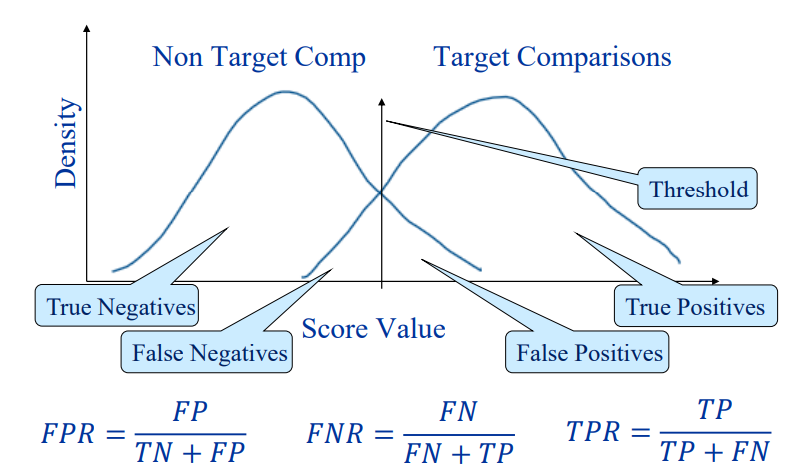
\includegraphics[width = 0.8\textwidth]{figs/medidas.png}
\caption{En la literatura se habla de Non Target Comparison en lugar de Negativos por la connotación. Normalmente hay un cierto solape entre las distribuciones target y non-target, produciendo así un error. El umbral de decisión se coloca dependiendo del error que se quiera priorizar (o si no se quiere priorizar ninguno).}
\end{figure}

\subsubsection{Curva ROC y AUC}
La curva ROC es una gráfica la tasa de verdaderos positivos (TPR; sensitividad) frente a la tasa de falsos positivos (FPR) para diferentes umbrales de decisión. La matriz de confusión solo tiene sentido cuando ya están las etiquetas y se ha definido un umbral, pero esto no es necesario para la curva ROC. 

El AUC (Área bajo la curva) mide el rendimiento general del clasificador. Un AUC cercano a 1 indica un buen rendimiento, mientras que un AUC cercano a 0.5 sugiere un rendimiento aleatorio.

\begin{figure}[h]
\centering
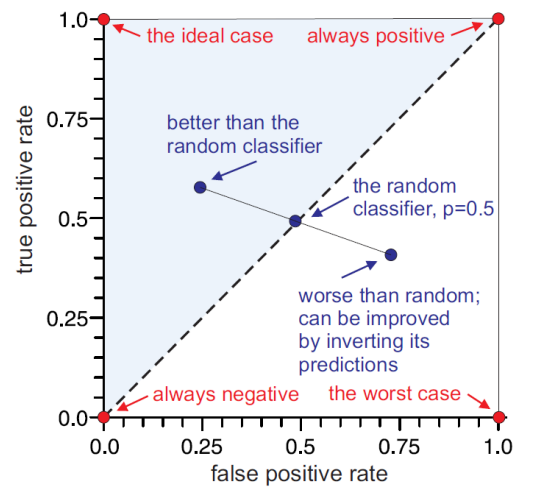
\includegraphics[width = 0.8\textwidth]{figs/roc.png}
\end{figure}

La curva ROC es útil para decidir el umbral de decisión óptimo, especialmente cuando se quiere priorizar la minimización de falsos negativos o falsos positivos.

\subsubsection{Métricas para regresión}
En problemas de regresión, las métricas comunes incluyen:
\begin{itemize}
\item \textbf{Error cuadrático medio (MSE)}:
$$MSE = \mathbb{E}[(h(\vec{X}; \Theta) - Y)^2] \approx \frac{1}{N} \sum^N_{n = 1}(h(\vec{x}_n;\Theta) - y_n)^2$$

\item \textbf{Error absoluto medio (MAE)}:
$$NMSE = \frac{MSE}{Var}$$
$$Var = \frac{1}{N} \sum^N_{n = 1} (y_n - \bar{y})^2$$

\item \textbf{Error cuadrático medio normalizado (NMSE)}:
$$MAE = \mathbb{E}[|h(\vec{X};\Theta) - Y|] \approx \frac{1}{N} \sum^N_{n = 1} |h(\vec{x}_n; \Theta) - y_n|$$
\end{itemize}

\subsection{Protocolos experimentales}
En general, tenemos un conjunto de datos que debemos dividir nosotros en dos conjuntos, uno de train y uno de test. 

\paragraph{Holdout}
Se divide el conjunto de datos en dos partes: una para entrenamiento (por ejemplo, 70\%) y otra para test (30\%). Problema: La partición puede no ser representativa si los datos no están bien distribuidos.

\paragraph{K-Fold Cross Validation}
El conjunto de datos se divide en $K$ subconjuntos (folds). El modelo se entrena $K$ veces, utilizando 
$K-1$ folds para entrenamiento y 1 fold para validación. El rendimiento final es el promedio de las $K$ iteraciones. Ventaja: Reduce la dependencia de una partición específica y proporciona una estimación más robusta del rendimiento.

\paragraph{Leave-One-Out}
 Caso extremo de K-Fold, donde $K=N$ (número de muestras). En cada iteración, se deja una muestra fuera para validación y se entrena con las $N-1$ restantes. Ventaja: Útil cuando el conjunto de datos es muy pequeño. Desventaja: Computacionalmente costoso y puede estar sesgado si hay outliers.

%25/02 - Daniel Hernández-Lobato
\section{Teoría de decisión}
En un problema de aprendizaje automático, trabajamos con datos observados (atributos) y etiquetas de clase. Por ejemplo:
\begin{itemize}
\item \textbf{Atributos}: una radiografía de un paciente.
\item \textbf{Etiquetas de clase}: si el paciente está sano o enfermo.
\end{itemize}

El objetivo es realizar \textbf{predicciones}: dado un nuevo paciente, asignarle una etiqueta (enfermo o sano) basándose en sus atributos. Para ello, asumimos que los datos observados se generan a partir de una \textbf{distribución de probabilidad conjunta} sobre los atributos y las etiquetas de clase. Una vez observados los atributos, utilizamos esta distribución para tomar decisiones sobre la asignación de etiquetas.

A partir de los datos observados, \textbf{inferimos} la distribución de probabilidad conjunta. Utilizamos la distribución inferida para asignar etiquetas a nuevos datos.

\subsection{Probabilidad condicional y regla de Bayes}
Para asignar una etiqueta a un nuevo dato, nos interesa la probabilidad condicional de la etiqueta dado los atributos observados, $p(C|x)$, donde:
\begin{itemize}
\item $C$: etiqueta de clase (por ejemplo, enfermo o sano).
\item $x$: atributos observados (por ejemplo, radiografía).
\end{itemize}

La \textbf{regla de Bayes} permite calcular esta probabilidad condicional:
$$p(C|x) = \frac{p(x|C) \cdot p(C)}{p(x)}$$
donde
\begin{itemize}
\item $p(x|C)$: probabilidad de observar los atributos $x$ dada la clase $C$ (verosimilitud).
\item $p(C)$: probabilidad a priori de la clase $C$ (por ejemplo, la fracción de la población que está enferma).
\item $p(x)$: probabilidad marginal de los atributos $x$ (constante de normalización).
\end{itemize}

Entre las reglas de probabilidad hay dos fundamentales:
\begin{itemize}
\item \textbf{Regla del producto}: la probabilidad conjunta de $x$ y $C$ es el producto de la verosimilitud y la probabilidad a priori.
$$p(x, C) = p(x|C) \cdot p(C)$$

\item \textbf{Regla de la suma}: la probabilidad marginal de $x$ se obtiene sumando (marginalizando) sobre todas las clases.
$$p(x) = p(x, C_1) + p(x, C_2)$$
\end{itemize}

\subsubsection{Ejemplo de probabilidades condicionales}
Consideremos un ejemplo con dos atributos: color de ojos y color de pelo. La siguiente tabla muestra las frecuencias observadas:
\begin{table}[h]
\centering
\begin{tabular}{ll|ll|}
\cline{3-4}
                                            &        & \multicolumn{2}{l|}{Pelo}         \\ \cline{3-4} 
                                            &        & \multicolumn{1}{l|}{Rojo} & Rubio \\ \hline
\multicolumn{1}{|l|}{\multirow{2}{*}{Ojos}} & Marrón & \multicolumn{1}{l|}{5}    & 10    \\ \cline{2-4} 
\multicolumn{1}{|l|}{}                      & Azul   & \multicolumn{1}{l|}{10}   & 20    \\ \hline
\end{tabular}
\end{table}

A partir de esta tabla, podemos calcular varias probabilidades
\begin{itemize}
\item Probabilidad marginal:
$$p(\text{ojos marrones}) = \frac{15}{45}$$

\item Probabilidad conjunta:
$$p(\text{ojos marrones, pelo rubio}) = \frac{10}{45}$$

\item Probabilidad condicional:
$$p(\text{ojos marrones}|\text{pelo rubio}) = \frac{10}{30}$$
\end{itemize}

\subsubsection{Probabilidad posterior para dos clases}
En un problema con dos clases ($C_1$ y $C_2$) se cumple que:
$$p(C_1|x) + p(C_2|x) = 1$$
Esto se debe a que, según la regla de Bayes:
$$p(C_1|x) = \frac{p(x|C_1) p(C_1}{p(x)}$$
$$p(C_2|x) = \frac{p(x|C_2) p(C_2}{p(x)}$$
Sumando ambas probabilidades:
$$p(C_1|x) + p(C_2|x) = \frac{p(x|C_1) \cdot p(C_1) + p(x|C_2) \cdot p(C_2)}{p(x)} = \frac{p(x)}{p(x)} = 1$$

\subsubsection{Ejercicios teorema de Bayes}
Estamos trabajando para una empresa que ha desarrollado una nueva prueba para detectar una enfermedad. La prueba se caracteriza por tener una alta probabilidad de dar positivo en personas enfermas. Sin embargo, a veces puede fallar como se indica en la siguiente tabla:

\begin{table}[h]
    \centering
    \begin{tabular}{|l|l|l|}
    \hline
        Test output & Is the person sick? & Probability \\ \hline
        + & Sick & 0.9 \\ \hline
        - & Sick & 0.1 \\ \hline
        + & Healthy & 0.05 \\ \hline
        - & Healthy & 0.95 \\ \hline
    \end{tabular}
\end{table}

Sean las dos etiquetas de clase $\mathcal{C}_0 \equiv \text{Healty}$ y $\mathcal{C}_1 \equiv \text{Sick}$ y $x$ el resultado de la prueba, es decir, las variables observadas. Por lo tanto, la tabla anterior proporciona todos los valores potenciales para las distribuciones condicionales de clase $p(x|\mathcal{C}_k)$.

\paragraph{Escenario 1} 
Supongamos que tenemos la misma probabilidad a priori de que una persona esté enferma o sana, es decir, $p(\mathcal{C}_1)=p(\mathcal{C}_0)=0,5$. 

\textit{Utiliza el teorema de Bayes para calcular la fracción de personas que están realmente enfermas a partir del número total de personas que son positivas según la prueba. Es decir, se pide calcular $p(\mathcal{C}_1|x=+)$.}
$$p(sick|+) = \frac{p(+|sick) \cdot p(sick)}{p(+)} =$$
$$ \frac{p(+|sick) p(sick)}{p(+, sick) + p(+, healthy)} = \frac{p(+, sick) p(sick)}{p(+|sick)p(sick) + p(+|healthy) p(healthy)}$$

Ahora rellenamos con los datos del enunciado y la tabla
$$\frac{0.9 \cdot 0.5}{0.9 \cdot 0.5 + 0.05 \cdot 0.5} = 0.95$$

\textit{Según los resultados obtenidos, ¿es muy buena la prueba desarrollada? ¿Por qué?}
Parece un buen test, ya que si es positivo, con un 95\% de probabilidad la persona realmente está enferma.

\paragraph{Escenario 2}
Supongamos ahora que la enfermedad es muy rara y que sólo afecta al 1\% de la población. Es decir, $p(\mathcal{C}_1)=0,01$. 

\textit{Utilice el teorema de Bayes para calcular la fracción de personas que están realmente enfermas a partir del número total de personas que son positivas según la prueba. Es decir, se le pide que calcule $p(\mathcal{C}_1|x=\text{+})$.}

$$p(sick|+) = \frac{p(+|sick) \cdot p(sick)}{p(+)} = $$
$$\frac{p(+|sick) p(sick)}{p(+, sick) + p(+, healthy)} = \frac{p(+, sick) p(sick)}{p(+|sick)p(sick) + p(+|healthy) p(healthy)}$$

Ahora rellenamos con los datos del enunciado y la tabla:
$$\frac{0.9 \cdot 0.01}{0.9 \cdot 0.01 + 0.05 \cdot 0.99} = 0.15$$

\textit{Según los resultados obtenidos, ¿es muy buena la prueba desarrollada? ¿Por qué? ¿Qué es lo que falla en la prueba en este escenario?}

Este test es malo, ya que con un test positivo, la probabilidad de estar enfermo es bastante baja. El problema está en los falsos positivos. Para mejorar el test, hay que reducir la probabilidad de los falsos positivos.

\textit{Calcula cuál es la tasa de falsos positivos necesaria, es decir, $p(x=\text{+}|\mathcal{C}_0)$, de la prueba para que al menos el 90\% de las personas que den positivo en la prueba estén realmente enfermas.}

Ahora queremos calcular $p(+ | healthy)$:
Sabemos que 
$$p(sick|+) = \frac{p(+|sick) \cdot p(sick)}{p(+)} = 0.9$$
y que:
$$p(+) = p(+, sick) + p(+, healthy)$$

Esto es igual a :
$$p(+) = p(+|sick) p(sick) + p(+|healthy) p(healthy)$$

Sustituyendo en función de la tabla del enunciado:
$$p(+) = 0.9 \cdot 0.01 + p(+|healthy) \cdot 0.99$$

Insertando esto en la primera fórmula:
$$0.9 = \frac{ p(+|healthy) \cdot p(sick)}{p(+)} = \frac{0.9 \cdot 0.01}{0.9 \cdot 0.01 +  p(+|healthy) \cdot 0.99}$$

Se puede pasar la parte de abajo de la fracción al otro lado:
$$0.9 \cdot 0.9 \cdot 0.01 + 0.9 \cdot p(+|healthy) \cdot 0.99 = 0.9 \cdot 0.01$$

Simplificando
$$0.9 \cdot p(+|healthy) \cdot 0.99 = 0.9 \cdot 0.01 - 0.9 \cdot 0.9 \cdot 0.01 $$
$$ p(+|healthy) = \frac{0.9 \cdot 0.01 - 0.9 \cdot 0.9 \cdot 0.01}{0.9 \cdot 0.99} = 10^{-3}$$
 
\paragraph{Escenario 3}
\textit{Supongamos ahora que disponemos de $T$ pruebas independientes para diagnosticar la enfermedad, pero que tienen las mismas características que las descritas en la tabla anterior. Como las pruebas son independientes, tenemos que }
$$ p(x_1=\text{+},x_2=\text{+},\ldots, x_T = \text{+}|\mathcal{C}_k)=\prod_{i=1}^T p(x_i=\text{+}|\mathcal{C}_k)$$
\textit{¿En cuántas de estas pruebas tiene que dar positivo una persona para que al menos el 90\% de las personas diagnosticadas como positivas estén realmente enfermas?}
$$p(sick | x_1 = +, ..., x_T = +) = 0.9$$

Se busca $T$. Tenemos la siguiente pista: $log(a^b) = b \cdot log(a)$ y $log(ab) = log(a) + log(b)$
$$p(sick | x_1 = +, ..., x_T = +) = p(+ | sick)^T = 0.9^T$$
$$p(sick | x_1 = +, ..., x_T = +) = 0.9 $$
$$0.9 = \frac{p(x_1 = +, ..., x_T = + | sick) \cdot p(sick)}{p(x_1 = +, ..., x_T = + | sick) \cdot p(sick) + p(x_1 = +, ..., x_T = + | healthy) \cdot p(healthy)}$$
$$p(healthy | x_1 = +, ..., x_T = +) = p(+ | healthy)^T = 0.05^T$$
$$0.9 = \frac{0.9^T \cdot 0.01}{0.9^T \cdot 0.01 + 0.05^T \cdot 0.99}$$
$$0.9 \cdot 0.9^T \cdot 0.01 + 0.9 \cdot 0.05^T \cdot 0.99 = 0.9^T \cdot 0.01$$
$$0.9 \cdot 0.05^T \cdot 0.99 = 0.9^T \cdot 0.01 - 0.9 \cdot 0.9^T \cdot 0.01$$
$$0.9 \cdot 0.05^T \cdot 0.99 = 0.9^T[0.01 - 0.9 \cdot 0.01]$$

Aplicando los logaritmos:
$$log 0.9 + T \cdot log 0.05 + log 0.99 = T \cdot log 0.9 + log(0.01 - 0.9 \cdot 0.01)$$
$$T log 0.05 - T log 0.9 = log(0.01 - 0.9 \cdot 0.01) - log 0.9 - log 0.99$$
$$T(log 0.05 - log 0.9) = \frac{log(0.01 - 0.9 \cdot 0.01) - log 0.9 - log 0.99}{log 0.05  log 0.9} = 2.3$$

%\section{Análisis discriminante}

%\section{Árboles de clasificación y vecinos cercanos}